\section{Minimum Spannign Tree}
Nei problemi \textbf{MSP}(Minimum Spannign Tree o albero di supporto minimo), dato un grafo non orientato $G=(V, E)$
con pesi $W_{ij} \forall (i, j) \in E$, si vuole determinare tra tutti gli alberi di supporto, quello con peso complessivo
$\sum_{(i,j) \in E_T} w_{ij}$ minimo.


\subsection{Algoritmo greedy per MSP}

\begin{enumerate}
    \item \textbf{Inizializzazione}: Si ordinano tutti gli $m = | E |$ archi del grafo in ordine crescente rispetto al peso degli archi
    \begin{itemize}
        \item Pongo $E_T = \emptyset$
        \item pongo $k = 1$
    \end{itemize}
    \item Se $|E_T| = |V| - 1$ mi fermo e restituisco l'albero $T = (V, E_T)$ come soluzione, altrimenti continuo.
    \item Se $e_t$(penso sia uno degli archi delli'insieme di archi $E$) non forma cicli con gli archi di $E_T$:
    \begin{itemize}
        \item pongo $E_T = E_T \cup \{e_k\}$
        \item altrimenti lascio invariato $E_T$
    \end{itemize}
    \item pongo $k = k + 1$ e torno al passo 2
\end{enumerate}

\subsubsection{Correttezza dell'algoritmo}
Per dimostrare che l'algoritmo greedy non è il migliore si fa una dimostrazione per assurdo,
cioè una volta terminato l'algoritmo greedy, si aggiunge un nuovo arco(formando cosi un ciclo), si leva 
un'arco per evitare il ciclo e si ricalcolano i pesi.

Se non vengono trovati percorsi migliori, greedy ha vinto, altrimenti si ottiene un nuovo MSP con peso minore.

\subsubsection{Complessità dell'algoritmo}
Solitamente l'operazione all'interno di un grafo è quella di ordinamento secondo l'ordine crescente degli archi.

Se siamo in presenza di grafi densi(numero di archi $O(|V|^2)$), l'operazione di ordinamento richiede
$O(|E|\log(|E|))$ operazioni.

\textbf{L'algoritmo greedy ha complessità}: $O(|E|\log(|E|))$.

\subsubsection{Foresta di supporto}
Chiamiamo foresta di support di un grafo, un grafo parziale privo di cicli, in particolare chiamiamo albero si 
supporto una foresta che ha solo una componente connessa.

\subsection{Algoritmo MST-1}
\begin{enumerate}
    \item \textbf{Inizializzo}: 
    \begin{enumerate}
        \item scelgo un nodo $v_1 \in V$
        \item pongo $U = \{v_1\}$
        \item $E_T = \emptyset$
        \item $c(v)$ conterra il nodo in $U$ più vicino a $v$
    \end{enumerate}
    \item se $U = V$ mi fermo
    \item seleziono $\bar{v}$ con peso minore($\bar{v}$ è il nodo di $V \backslash U$ più vicino a $U$)
    \item pongo $U \cup {\bar{v}}$ e $E_T = E_T \cup \{(\bar{v}, c(\bar{v}))\}$
    \item $\forall v \in V \backslash U$ se il peso di $v\bar{v}$ è minore del peso di $vc(\bar{v})$, pongo $c(v) = \bar{v}$ e torno al passo 2
\end{enumerate}

\subsubsection{Complessità dell'algoritmo}
Complessità: $O(|V|^2)$

Molto buono per grafi densi.

\subsection{Algoritmo MST-2}

\begin{figure}[H]
    \centering
    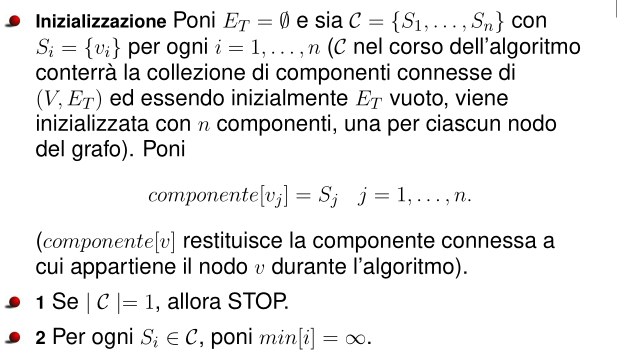
\includegraphics[width=0.6\linewidth]{img/Screenshot from 2022-06-01 11-25-45.png}
\end{figure}

\begin{figure}[H]
    \centering
    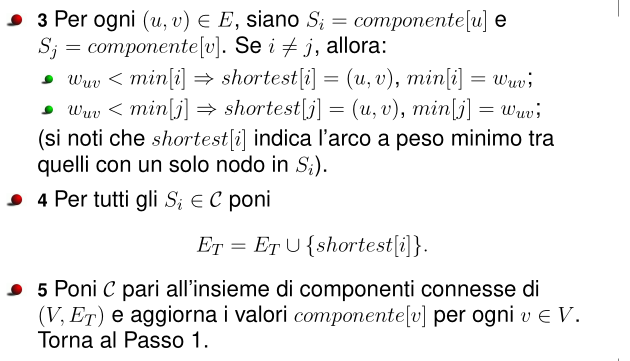
\includegraphics[width=0.6\linewidth]{img/Screenshot from 2022-06-01 11-26-45.png}
\end{figure}

\subsubsection{Complessità}
Complessità: $O(|E|\log(|V|))$


\section{Shortest Path}
Nei problemi di cammino a costo minimo, dato un grafo orientato $G=(V, A)$ che ha un costo per ogni arco,
si vuole individuare un percorso con il mino costo possibile.

\subsection{Algoritmi per Shortest Path}
usiamo due algoritmi:
\begin{itemize}
    \item \textbf{Dijksta}: valido solo se i costi dei percorsi sono maggiori o uguali a 0 per ogni percorso.
    \item \textbf{Floyd-Warshall}: valido anche er distanze negative
\end{itemize}


Per i prossimi algoritmi si supporrà che:
\begin{itemize}
    \item il peso dei percorsi non appartenenti all'insieme degli archi sia $+ \infty$
    \item la cardinalità dei vertici è $n$
\end{itemize}

\subsection{Algoritmo di Dijkstra}
